\documentclass[border=3pt,tikz]{standalone}
\usepackage{amsmath,amssymb}
\usepackage{bm} % math bold
\usepackage[outline]{contour} % glow around text
\contourlength{1.2pt}

\usepackage{tikz}
\usetikzlibrary{patterns}
\tikzset{>=latex}

\begin{document}

% CRITICAL REGION
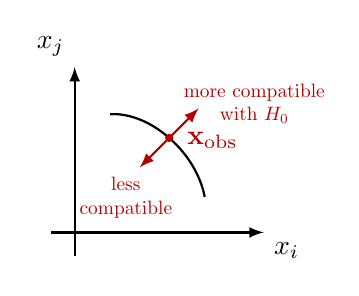
\begin{tikzpicture}[scale=1.5]
  
  \coordinate (L)  at ( 0.3,  1.0  );
  \coordinate (M)  at ( 0.8,  0.8  );
  \coordinate (R)  at ( 1.1,  0.3  );
  
  % AXES
  \draw[->,thick]
    (-0.2,0) -- (1.6,0) node[anchor=north west] {$x_i$};
  \draw[->,thick]
    (0,-0.2) -- (0,1.4) node[anchor=south east] {$x_j$};
  
  % BORDER
  \draw[thick] plot[smooth,tension=1.2]
    coordinates {(L) (M) (R)};
  \draw[thick,->,red!70!black]
    (M) --++ ( 0.25, 0.25) node[above right=-8pt,scale=0.7,align=center] {more compatible\\with $H_0$};
  \draw[thick,->,red!70!black]
    (M) --++ (-0.25,-0.25) node[left=5pt,below=1pt,scale=0.7,align=center] {less\\compatible};
  \fill[radius=1pt,red!70!black]
    (M) circle node[below=1pt,right=3pt] {$\mathbf{x}_\text{obs}$};
  
\end{tikzpicture}

\end{document}